% !TEX root = rob1.tex
\chapter{Autonome Roboter}

\section{Überblick}
\subsection{Fähigkeiten eines autonomen Robotersystems}
\begin{figure}[!h]
    \centering
    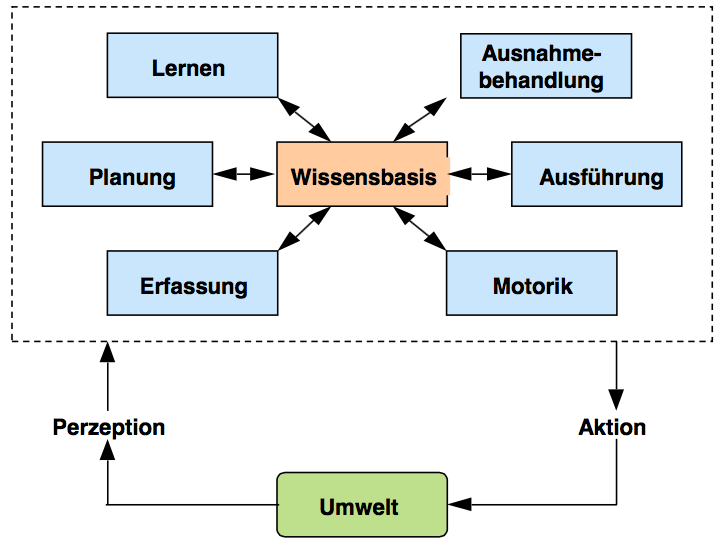
\includegraphics [scale=0.3]{faehig}
\end{figure}

\subsection{Architekturübersicht}
\begin{figure}[!h]
    \centering
    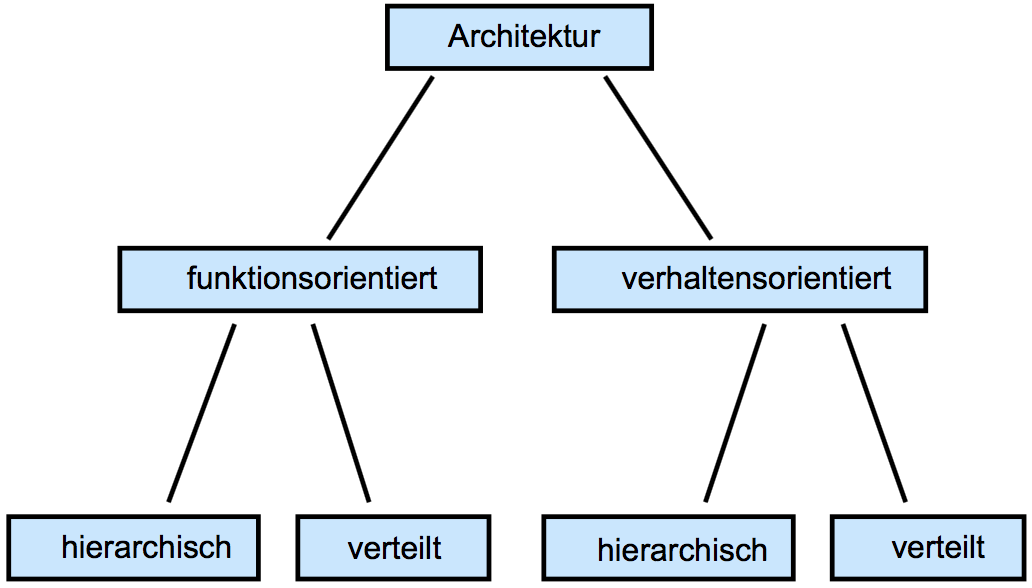
\includegraphics [scale=0.3]{architektur}
\end{figure}

\section{Funktionsorientierte Architektur}
\subsection{Genereller Aufbau}
\begin{figure}[!h]
    \centering
    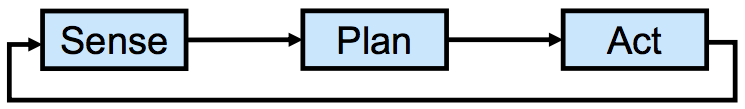
\includegraphics [scale=0.8]{generel}
    \caption{Sense Plan Act Architektur}
\end{figure}

\begin{compactitem}
    \item Unidirektionaler Informationsfluss
    \item Schlecht für dynamisch Umgebung, Interaktion
    \item Einfacher Aufbau
\end{compactitem}

\subsection{Hierarchische funktionsorientierte Architekturen}
\subsection{Verteilt funktionsorientierte Architekturen}
\section{Verhaltensorientierte Architektur}
